\section{Diskussion}
\label{sec:Diskussion}
Besonders augenfällig ist der plötzliche Sprung der aufgenommen Messwerte bei der Messung mit grünem Licht, siehe \autoref{fig:grun}.
Der Sprung kommt wahrscheinlich von einer Erschütterung der Messapparatur, welche mit sehr empfindlichen Koaxialkabeln aufgebaut ist.
In der \autoref{fig:gelba} wurden wegen des Sättigungswertes, der sich für hohe Beschleunigungsspannungen einsetzt, nicht alle Messwerte in die Ausgleichsrechnung einbezogen.
Der Beginn des linearen Zusammenhangs ist nur grob einschätzbar und durch eine leicht andere Wahl, könnten die errechneten Werte noch genauer oder ungenauer werden.
Die Werte an sich zeigen vor und nach dem Sprung das erwartete Verhalten, sodass ein weiterer Fehler durch die Geräte auszuschließen ist.
In der Auswertung fällt auf, dass die Messunsicherheiten der bestimmten Größen meist einen höheren Betrag haben als die eigentlichen Größen. 
Bei den Parameter der linearen Fits ist dies damit zu erklären, dass die gemessenen Werte in dem aufgetragenen Zusammenhang kein lineares Verhalten zeigt, also die Linearität eher erzwungen ist.
Die fällt besonders bei der \autoref{fig:b} auf, wobei hier die geringe Anzahl der Punkte zu beachten ist. 
Hier wurde mit dem Fit das Verhältnis $\frac{h}{e_0}$ ermittelt. 
\begin{align*}
    \frac{h}{e_0}_{\text{theo}} &= \SI{4.135e-15}{\volt\second}\\
    \frac{h}{e_0}_{\text{exp}} &= \SI{3.5(24)e-15}{\volt\second}
\end{align*} 
Damit beträgt die Abweichung vom Literaturwert $\SI{20}{\percent}$, welches in Anbetracht der anderen Werte ein recht gutes Ergebnis ist.

\section{Anhang}
\begin{figure}
    \centering
    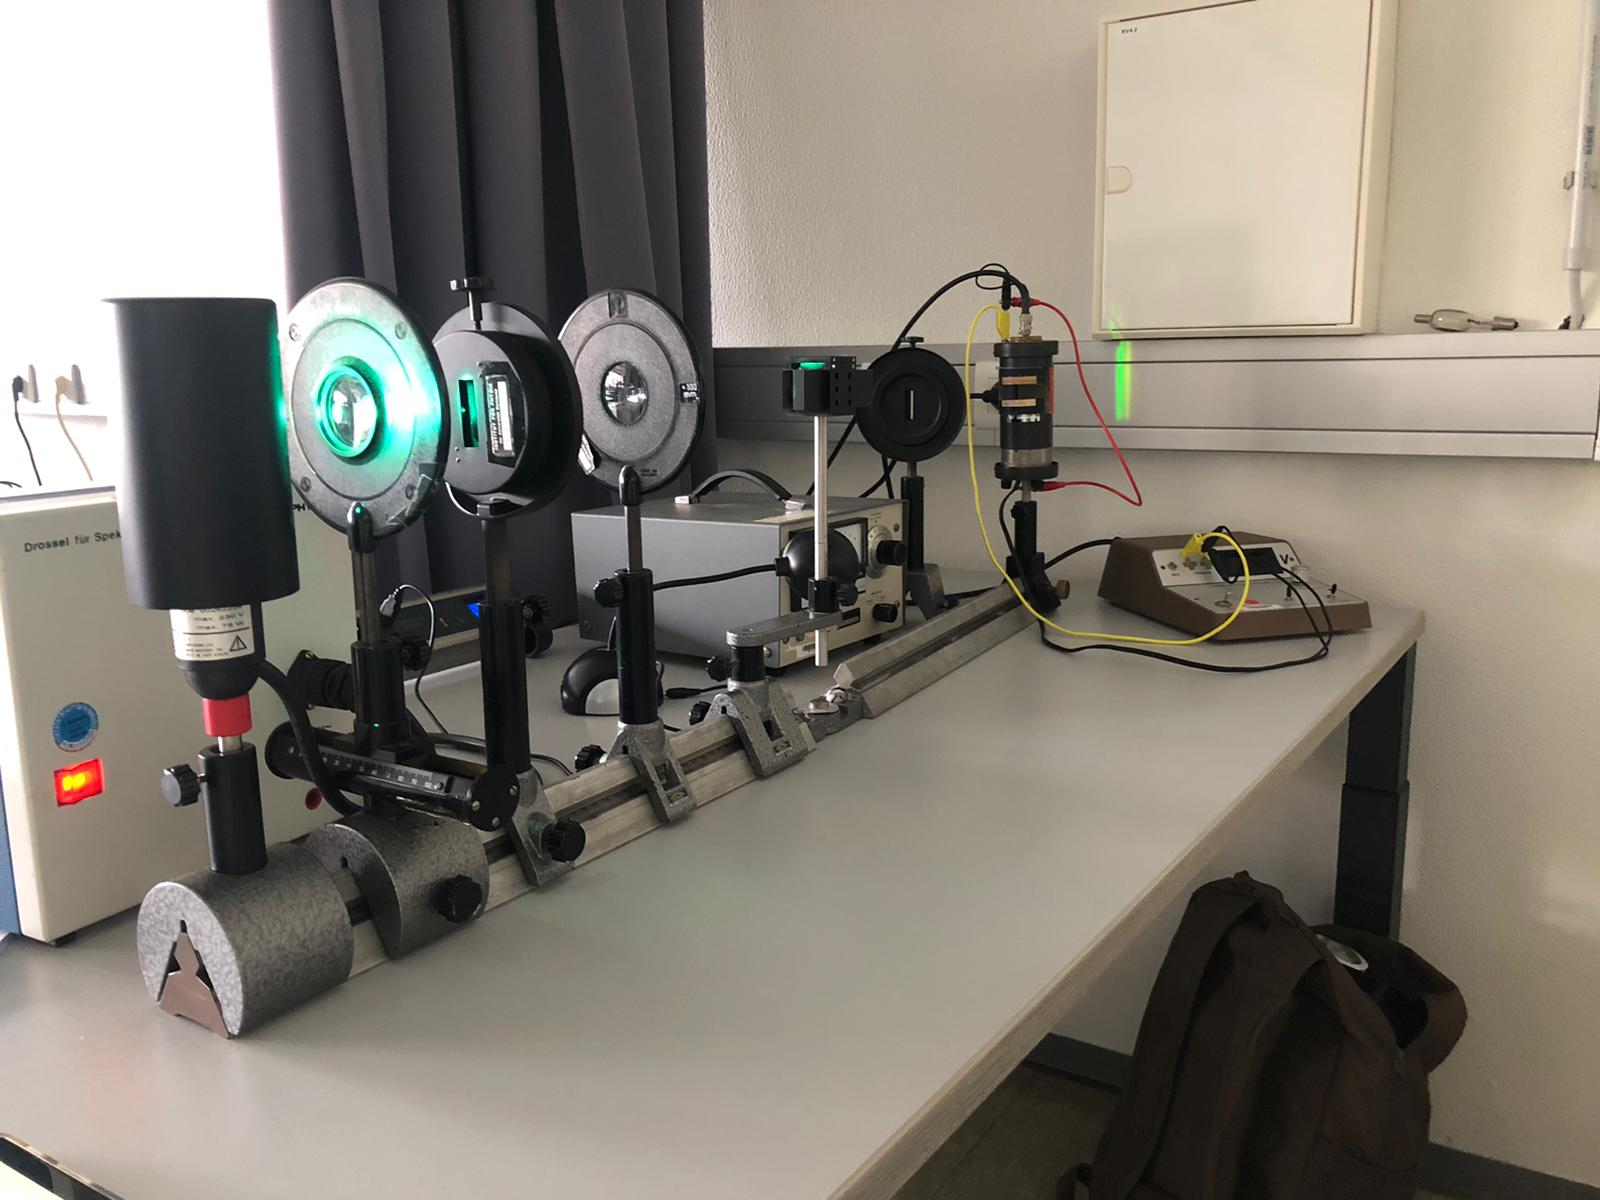
\includegraphics[width=\textwidth]{content/aufbaufotot.jpeg}
    \caption{Der Aufbau der Messapparatur. 
    Links ist die Hg-Dampflampe zu sehen, auf der Schiene folgen dann von links nach rechts eine Linse, ein Spalt, und eine weitere Linse.
    Anschließend folgt ein Prisma, welches das Licht aufspaltet.
    Auf einem weiteren Schienenteil, welches sich auf einem Kreisbogen relativ zu dem anderen Teil bewegen lässt, befindet sich die Photozelle.
    Hinter dem Stab, der das Prisma trägt, ist das Pico-Amperemeter zu sehen.
    Das bräunliche Gerät, aus dem das gelbe Kabel kommt, ist der Generator für die Gegenspannung.}
    \label{fig:fotoaufbau}
\end{figure}
\begin{figure}
    \centering
    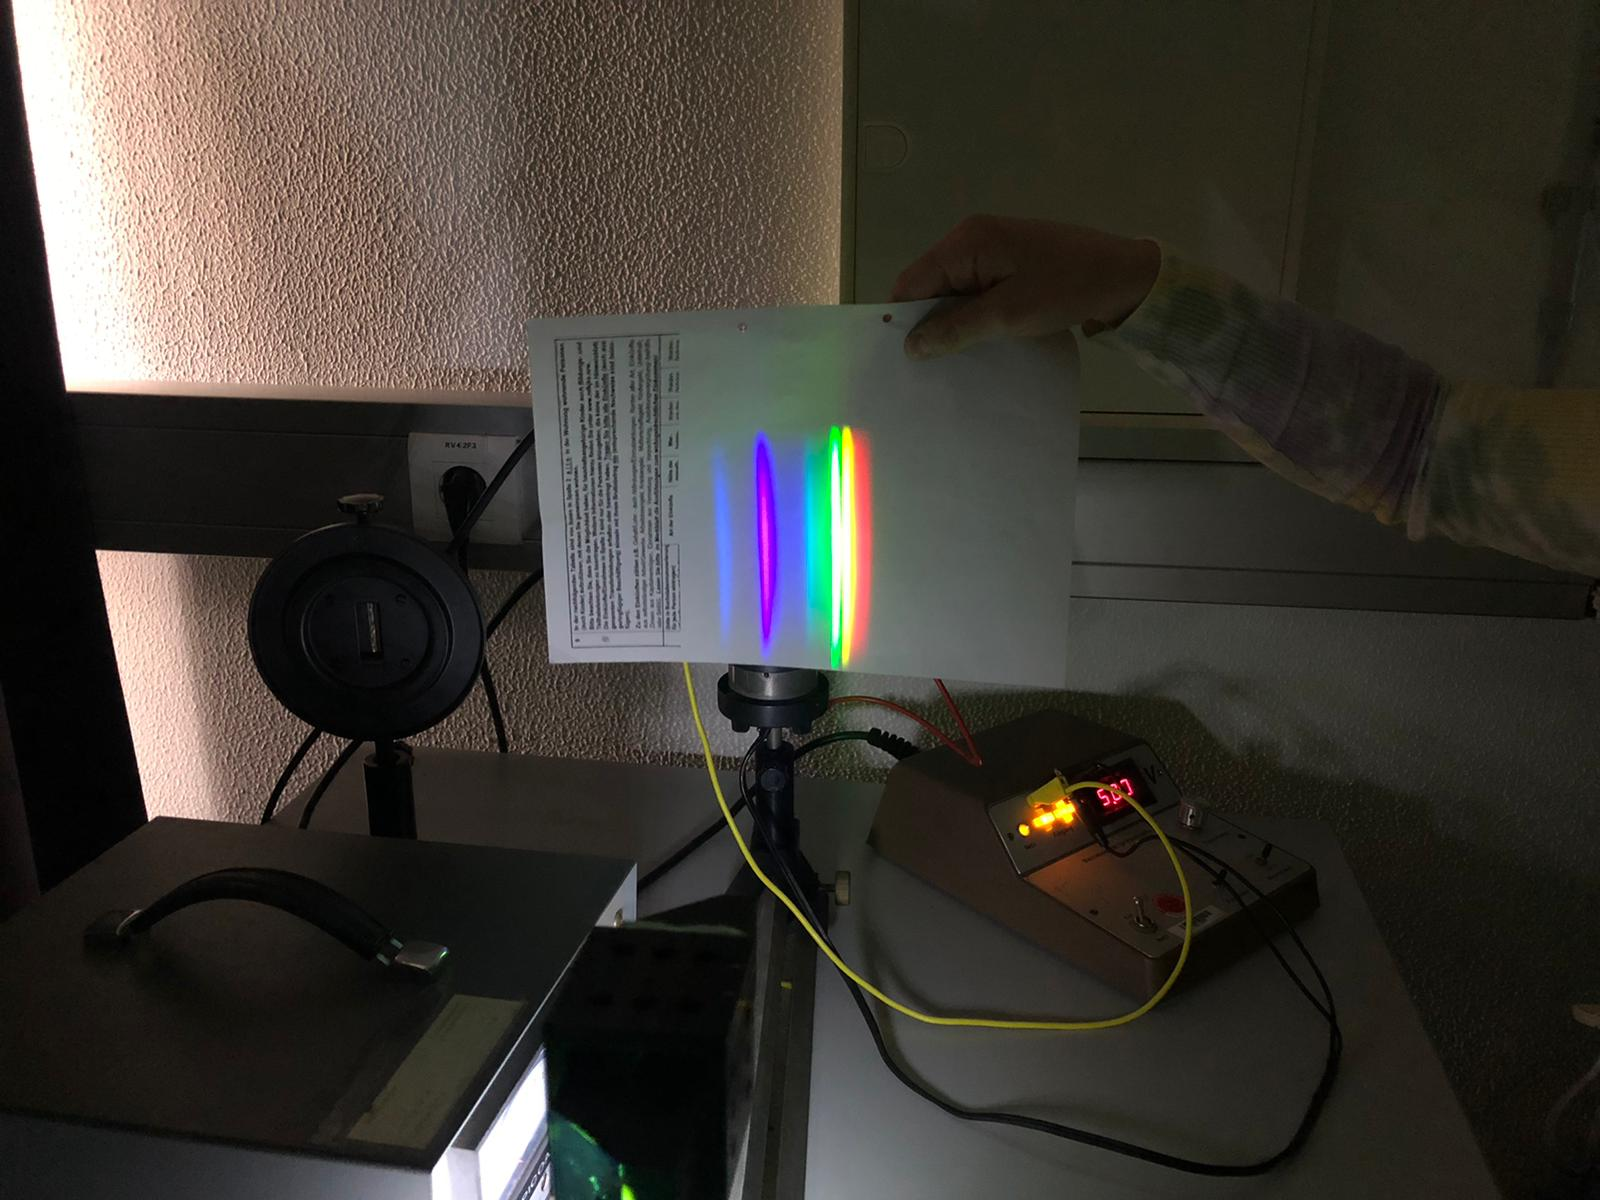
\includegraphics[width=\textwidth]{content/farben.jpeg}
    \caption{Die vom Prisma aufgespalteten Spektrallinien der Hg-Dampflampe.}
    \label{fig:fotofarben}
\end{figure}
\begin{figure}
    \centering
    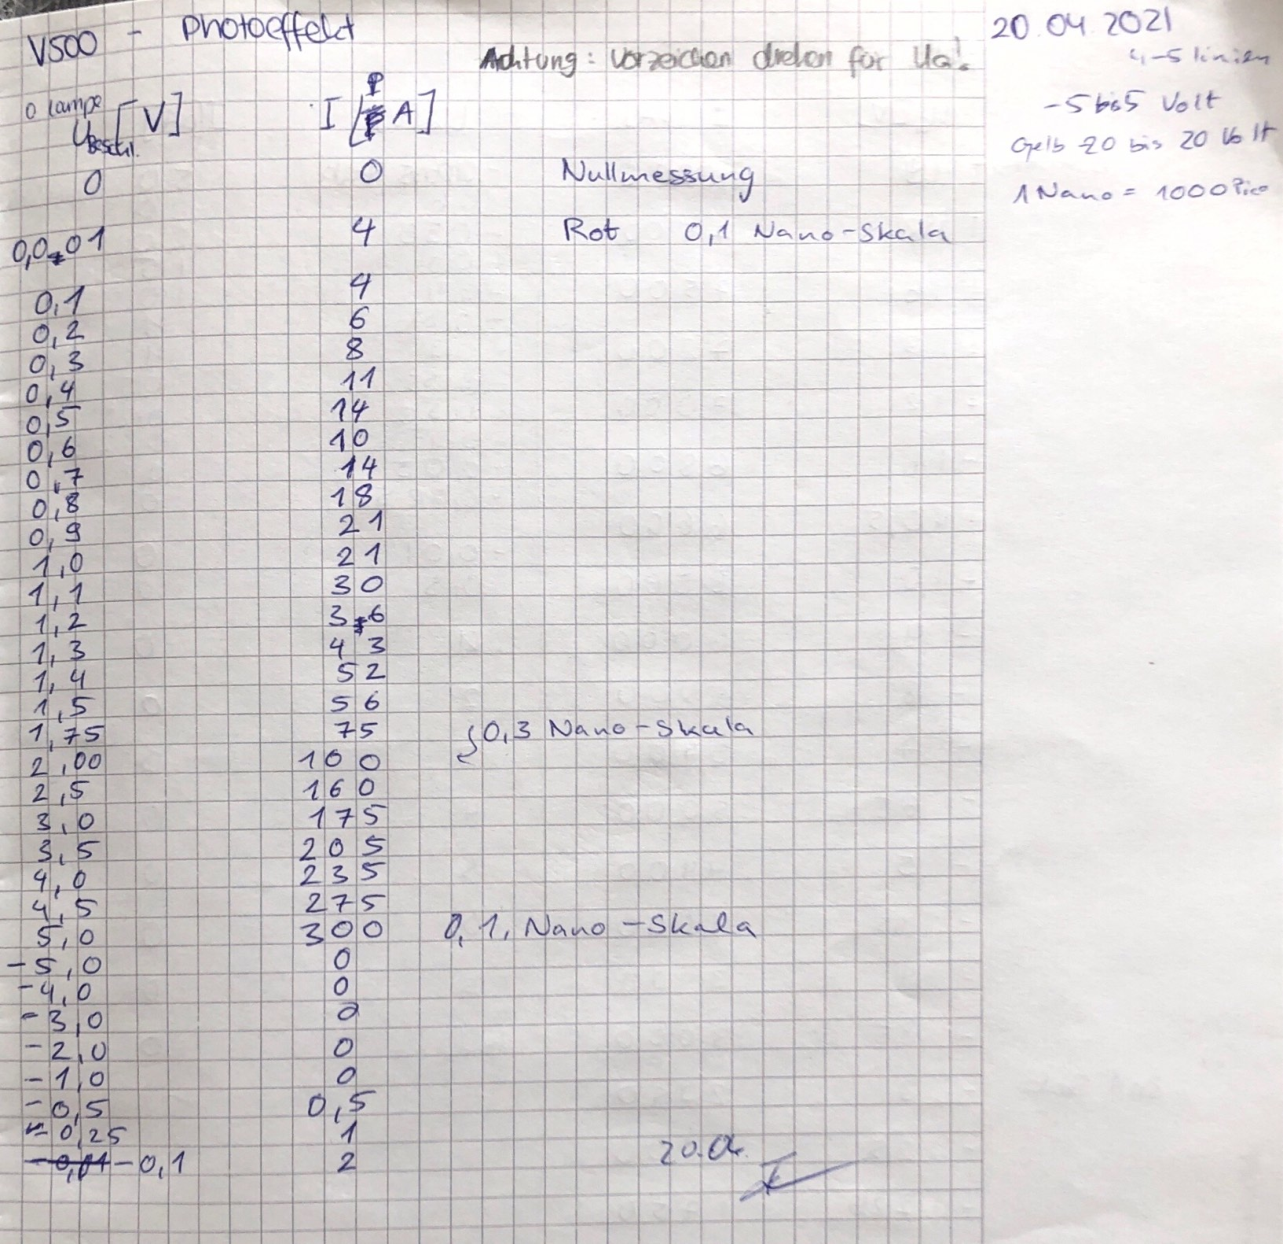
\includegraphics[width=\textwidth]{content/photorot.pdf}
\end{figure}
\begin{figure}
    \centering
    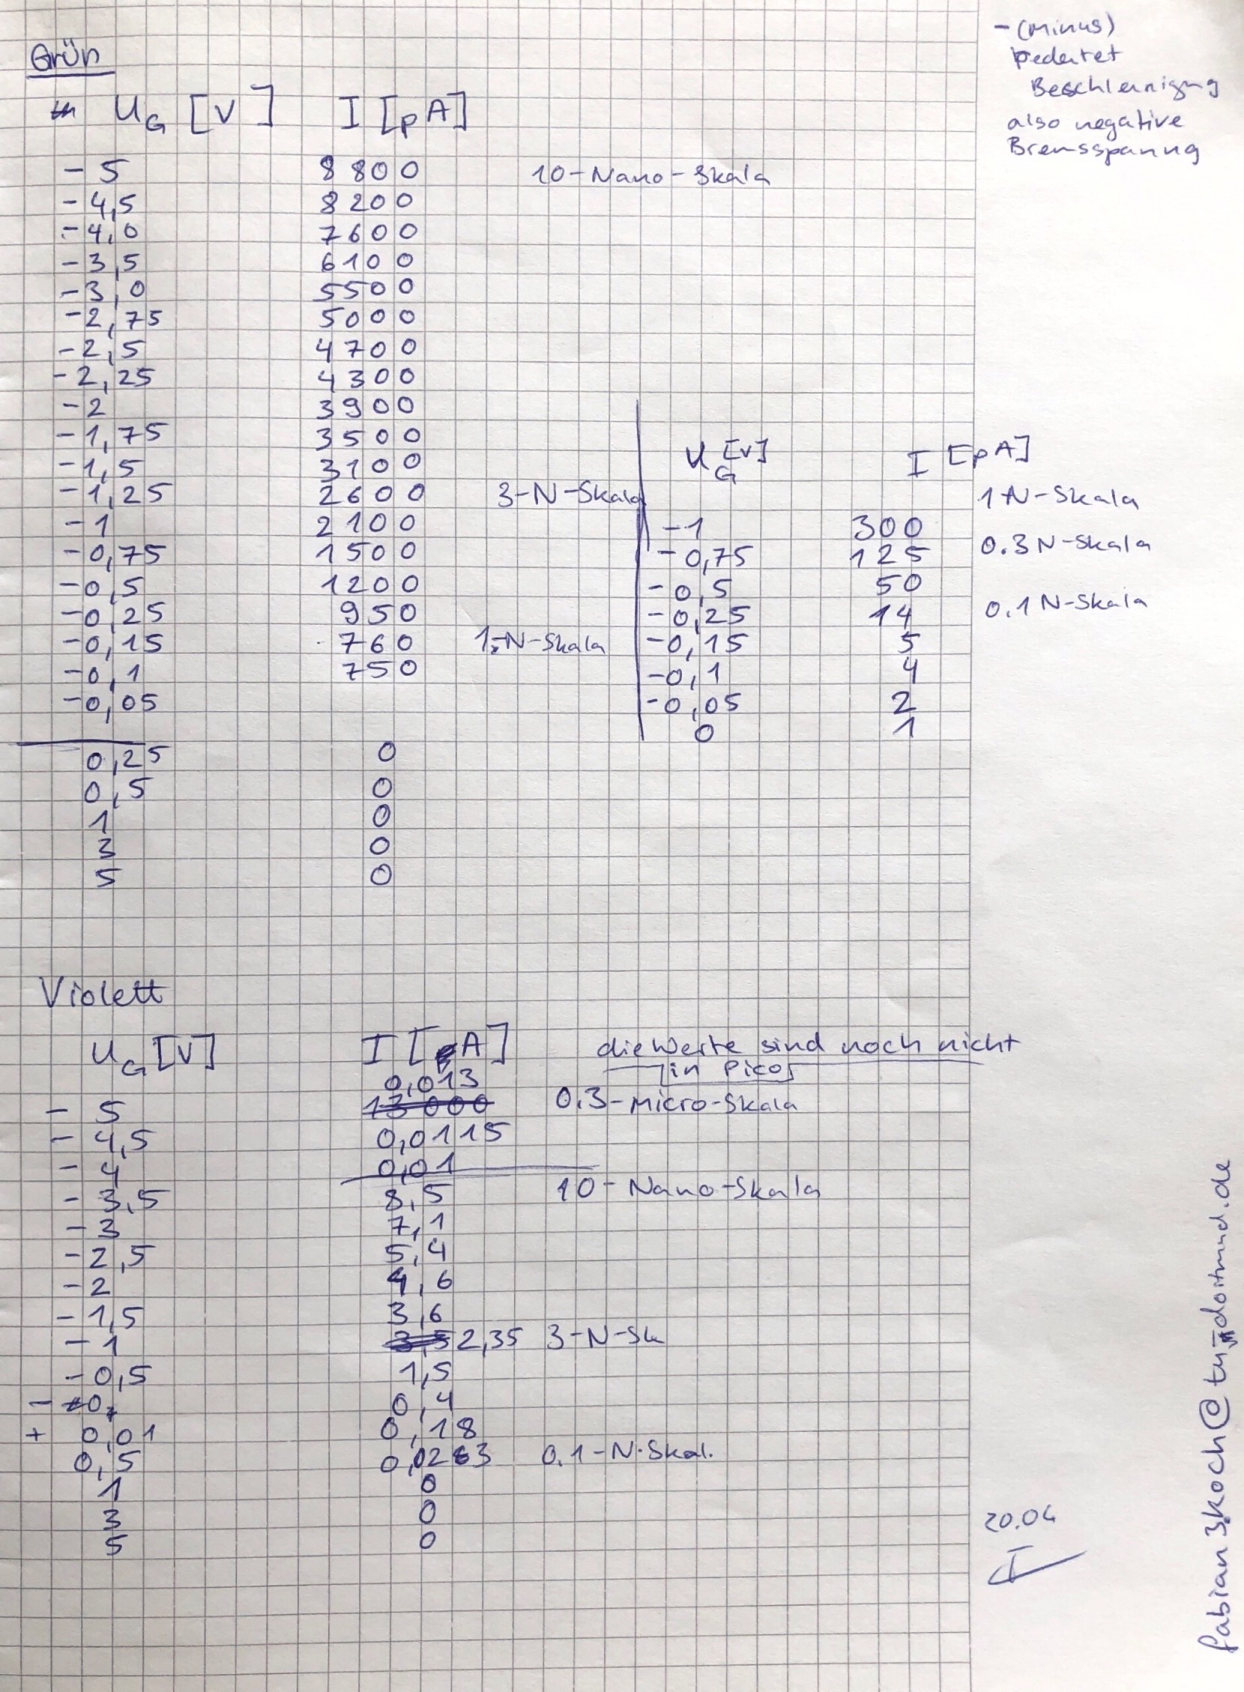
\includegraphics[width=\textwidth]{content/photogrunvio.pdf}
\end{figure}
\begin{figure}
    \centering
    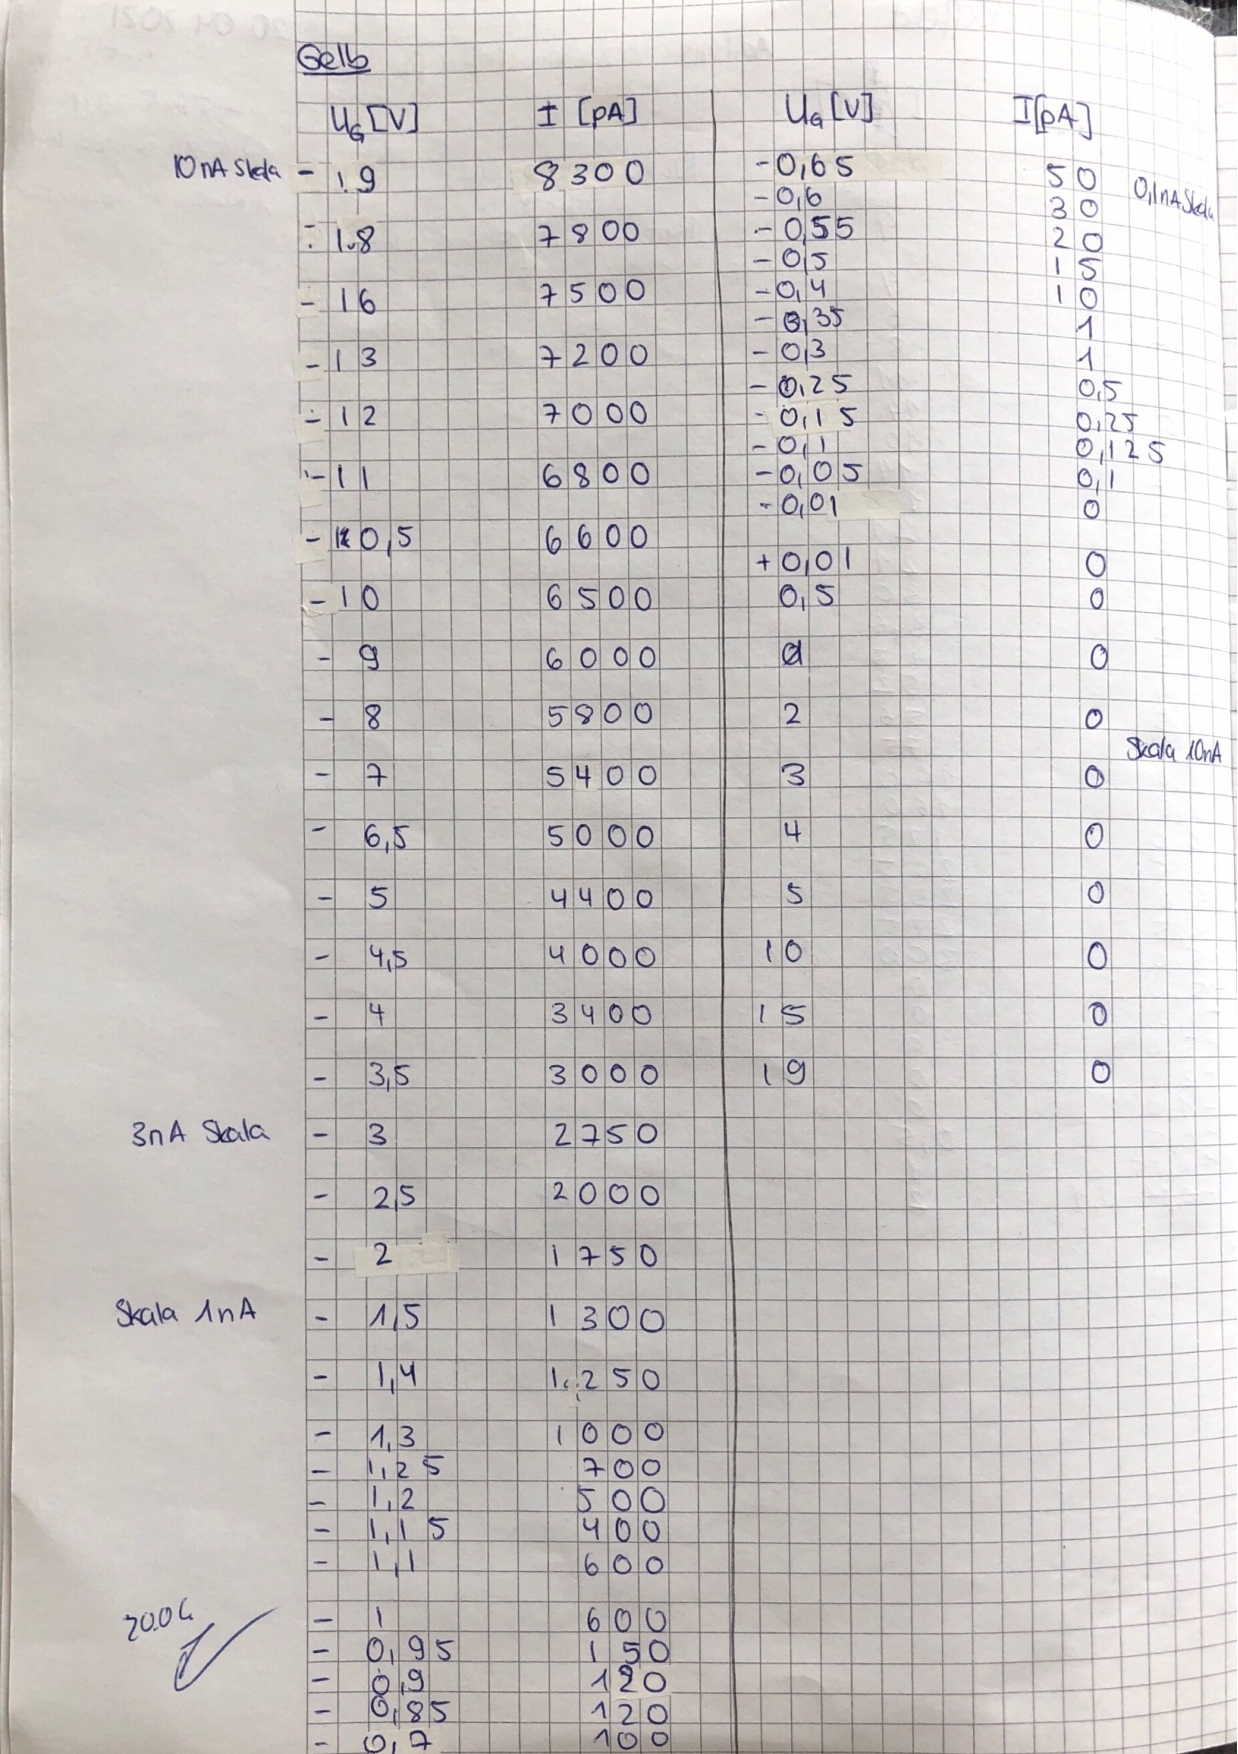
\includegraphics[width=\textwidth]{content/photogelb.pdf}
\end{figure}

    
